\chapter{Universal Constructions I}
We've been hinting at the utility of knowing that categories that have certain
special objects in them. For example, if we want to give a category that lets us
validate equations of programming languages, that category will need to be able 
to represent the many features that programs might have: products, sums, 
functions, etc. Here we will introduce the essential idea of a \textbf{universal 
construction} that characterizes when categories contain these special objects.

\section{Terminal objects \& the unit type}
Recall that when designing categorical semantics for programming languages we
associate types and typing contexts with objects in the category and terms with
morphisms. Concretely, if we have a well-typed term $\Gamma \vdash e : A$,
its interpretation $\dbracket{\Gamma \vdash e : A}$ is a morphism
$\dbracket{\Gamma} \xrightarrow{\dbracket{e}} \dbracket{A}$.
Previously, we showed how \(\FinSet\) can be used to give an interpretation 
to \ref{lang:calc} programs by associating types like the unit type $\plUnit$
with special sets, like a set containing only a single element $\{\star\}$.
But, what if we want to see if categories other than $\FinSet$ can give give a 
reasonable interpretation for $\plUnit$?

To proceed, let's pick a particular object $\dbracket{\plUnit}$ 
in a category $\calC$ and explore what properties it needs to have in order 
to be ``$\plUnit$-like'':
\begin{itemize}
  \item \textbf{Fact 1, Introduction rules}: It must be possible in any typing context to
  produce a value of type $\plUnit$.  This tells us that for any context
  $\Gamma$, there must exist a $\calC$-morphism
  $\dbracket{\Gamma} \to \dbracket{\plUnit}$.
  For example, it must 
  be the case that 
  $\dbracket{\Gamma} \xrightarrow{\dbracket{\plunit}} \dbracket{\plUnit}$.

  \item \textbf{Fact 2, Equational laws}: Since \ref{lang:calc} has no effects, 
  it is the case that if $\Gamma \vdash e : \plUnit$, then it is indistinguishable 
  from the term $\plunit$. This is called \textbf{eta equality}, and we write
  this as $e \equiv \plunit$.\footnote{The symbol ``$\equiv$'' means ``is
  equationally equal to''.} Eta equality is an equational law that characterizes
  how a $\plUnit$ term must behave. Now for an insight: \emph{these equational
  laws are translated into morphism equalities}. It must be that, for any
  morphism $\dbracket{\Gamma} \xrightarrow{\dbracket{e}} \dbracket{\plUnit}$, it
  is the case that $\dbracket{e} = \dbracket{\plunit}$.  In other words, the
  morphism $\dbracket{\Gamma} \xrightarrow{\dbracket{\plunit}} \plUnit$ must be
  unique.
\end{itemize}

These two properties can be packaged up into a nice concise definition:

\begin{definition}[Terminal object]  \label{def:terminal-object}
  Let $T$ be an object in a category $\calC$. 
  An object $T$ in $\calC$ is called a terminal object
  if
  \begin{itemize}
  \item
    for every object \(\Gamma\) in \(\calC\)
    there is a morphism \(\Gamma \xrightarrow{\angled{}} T\);
  \item
    for every morphism \(\Gamma \xrightarrow{f} T\)
    it holds that \(f = \angled{}\).
  \end{itemize}
\end{definition}

Let's pause to remark on the three categorical interpretations 
of terminal objects $T$:
\begin{itemize}
  \item Graphically, an object is terminal if (1) there is an arrow from 
  every other object to it, and (2) it ``thins all parallel
  arrows'', meaning that if we have a situation like the following for 
  and morphisms $X \xrightarrow{f} T, X \xrightarrow{g} T$:
  \begin{align*}
    % https://tikzcd.yichuanshen.de/#N4Igdg9gJgpgziAXAbVABwnAlgFyxMJZABgBpiBdUkANwEMAbAVxiRABUQBfU9TXfIRRkAjFVqMWbABrdxMKAHN4RUADMAThAC2SEdRwQkZEACMYYKEgC0AZhMM65hgAV+eAmw1ZFACxwg1PTMrIggity8IJo6egZGiCbmlkj21I7ObtgeQiAMMGoBQZKh0XJcQA
\begin{tikzcd}
  T                                                       \\
  X \arrow[u, "g"', bend right] \arrow[u, "f", bend left]
  \end{tikzcd},
  \end{align*}
  then we know that $f = g$.
  In other words, there is a unique morphism \(\Gamma \to T\) for every \(\Gamma\):
  \begin{center}
% https://tikzcd.yichuanshen.de/#N4Igdg9gJgpgziAXAbVABwnAlgFyxMJZABgBpiBdUkANwEMAbAVxiRAEEQBfU9TXfIRQBGclVqMWbACrdxMKAHN4RUADMAThAC2SMiBwQkokAyxhWiEHAhmoIagzoAjGAwAK-PATYMYanAcJZksQAB0wmAAPLDgcOABCOS4gA
\begin{tikzcd}
  A \arrow[r, "\exists!"] & T
  \end{tikzcd}
\end{center}
  \item The order-theoretic perspective is that the terminal object 
  is the ``greatest object'' in the category.
  \item The algebraic perspective
    says that, for every object \(\Gamma\),
    the equation \(f = f\) has a unique solution
    in the unknown \( \Gamma \xrightarrow{f} T\).
\end{itemize}

We say a category \textbf{has terminal objects} if there is an object in the
category that is a terminal object. This is our first example of a 
\textbf{universal construction}, which are special objects in categories 
characterized by their morphisms into them. We will see how universal 
constructions can be used to give interpretations to all the type 
formers we have seen so far. But, we can already see their utility: 
whether or not a particular category admits certain universal constructions
will immediately inform us of that category's suitability for modeling 
certain language properties.

\subsection{$\FinSet$ has terminal objects, isomorphisms}
We saw in previous lectures that we could use the singleton set 
$\{\star\}$ to give an interpretation to $\plUnit$ in $\FinSet$.
We can easily prove that $\{\star\}$ is a terminal object:
\begin{theorem}
  The singleton set $\{\star\}$ is terminal in $\FinSet$.
\end{theorem}
\begin{proof}
  \begin{itemize}
    \item Existence: The map $\_ \mapsto \{\star\}$ has the required type.
    \item Uniqueness: Suppose we have two morphisms $A \xrightarrow{f} \{\star\}$ and
    $A \xrightarrow{g} \{\star\}$. 
    Then by function extensionality we immediately have that $f = g$ 
    as set-functions, and so they are equal as $\FinSet$ morphisms.
  \end{itemize}
\end{proof}

Now you can observe the above proof and see that it immediately 
works for \emph{any} choice of singleton set: does this mean that $\FinSet$
has \emph{many terminal objects?} Yes, and no. \emph{Yes}, in the sense 
that there are indeed many valid choices of terminal object; but \emph{no}, 
in the sense that the choice itself does not (\emph{should} not!) actually 
matter. We capture this by the notion of isomorphism:

\begin{definition}[Isomorphism of objects]
  \sloppy
  Two objects $A$ and $B$ in a category $\calC$ are isomorphic if 
  there exist morphisms $A \xrightarrow{f} B$ and $B \xrightarrow{g} A$
  such that (1) $g \circ f = \id_A$ and (2) $f \circ g = \id_B$.
\end{definition}

We can immediately see that any two singleton sets in $\FinSet$ are isomorphic:
this proof is straightforward. What might be surprising is that this 
fact is true for all terminal objects:

\begin{theorem} \label{thm:terminal-object-unique}
  Terminal objects are unique up to isomorphism.
\end{theorem}
\begin{proof}
  Let $X$ and $Y$ be terminal objects in some category $\calC$. 
  Then there exists a pair of unique morphisms between them:

  \begin{center}
 % https://tikzcd.yichuanshen.de/#N4Igdg9gJgpgziAXAbVABwnAlgFyxMJZABgBpiBdUkANwEMAbAVxiRAA0QBfU9TXfIRQBGclVqMWbAJrdxMKAHN4RUADMAThAC2SMiBwQkokACMYYKEgDM++s1aIQAQjXdeITTuPVDe6uaWNnaSji6KclxAA
\begin{tikzcd}
  X \arrow[r, "!f", bend left] & Y \arrow[l, "!g", bend left]
  \end{tikzcd} 
\end{center}
By the fact that $X$ and $Y$ are terminal, they must also have unique identity
morphisms $\id_X$ and $\id_Y$. Then by the uniqueness of identity we have that $f \circ g = \id_X$ and $g \circ f = \id_Y$.
\end{proof}

This provides some evidence that the choice of terminal object does not matter.
  But are we done? Suppose we had two terminal objects \(T\) and \(T'\).
  By the above argument, we have that these two objects are isomorphic.
  But now another potential choice arises: what if there are multiple different
  \emph{isomorphisms} between \(T\) and \(T'\)?
  Then it could be that the choice to use \(T\) instead of \(T'\)
  may implicitly come with a choice of specific isomorphism as well.

  Luckily, terminal objects satisfy a stronger property
  which ensures that one's choice is terminal object is truly irrelevant.

\begin{proposition}
  Terminal objects are unique up to \emph{unique} isomorphism.
  That is, if \(T\) and \(T'\) are both terminal,
  then there is exactly one isomorphism
  \((f:T\to T',g:T'\to T)\)
  between \(T\) and \(T'\).
\end{proposition}
\begin{proof}
  Both \(f\) and \(g\), as constructed in the proof of
  \Cref{thm:terminal-object-unique},
  are the only possible morphisms \(T \to T'\) and \(T'\to T\)
  respectively. Thus they together form the only isomorphism
  between \(T\) and \(T'\).
\end{proof}

Later on, when we have the language for it, we will show that
all universal constructions are unique up to unique isomorphism
in this sense, and hence free of non-canonical choices.


% \subsection{Terminal objects for preorders}
% Universal constructions are one of the engines for analogy in category theory:
% very different-seeming concepts can be cast as instances of the same 
% universal construction, which can bring clarity to what each of those disparate 
% concepts means. When cast order-theoretically, the terminal object can 
% be thought of as ``the greatest object in a category.''
% % The first instance we will see of a universal construction is a \textbf{terminal 
% % object}, which can be thought of as ``the largest object in a category'' if one 
% % recalls the preorder intuition of morphisms. 

% An element of a preorder is the largest if it is greater than every other 
% element: i.e., there exists a morphism from every other element to it.
% This definition works for a general category: one could say an object is 
% largest if there exists a morphism from every other object into it.
% This characterization however doesn't take into account that there 
% can be more than 1 morphism between any two objects in a category: intuitively, 
% this means that one object can be greater than another in more than one way.

\section{Products}
Next we want to interpret product types $A \times B$. As before with the 
unit type, the typing rules for products forces the existence of certain morphisms,
and the equational theory of products forces equalities of certain morphisms.
The  introduction rule that describes how to create new products is:
\begin{mathpar}
\inferrule
    {\Gamma\vdash M : A
      \\
    \Gamma\vdash N : B
    }
    {\Gamma \vdash \plpair{M}{N} : A \pltimes B}~(\textsc{T-Pair})
\end{mathpar}
The elimination rules that break apart products are:
\begin{mathpar}
\inferrule
    {\Gamma\vdash M : A \pltimes B}
    {\Gamma \vdash \plfst{M} : A}~(\textsc{T-Fst})
\and
\inferrule
    {\Gamma\vdash M : A \pltimes B}
    {\Gamma \vdash \plsnd{M} : B}~(\textsc{T-Snd})
\end{mathpar}

These rules imply the existence of several morphisms that characterize 
what it means for for a special object $\dbracket{A \times B}$ to be a 
product. Reading off from the rules:
\begin{itemize}
  \item The \textsc{T-Pair} rules says that if there are 
  two morphisms $\dbracket{\Gamma} \mor{\dbracket{M}} \dbracket{A}$ and 
  $\dbracket{\Gamma} \mor{\dbracket{N}} \dbracket{B}$, 
  then there is a morphism $\dbracket{\Gamma} \mor{\dbracket{\langle M, N \rangle}} 
  \dbracket{A \times B}$.
  \item The \textsc{T-Fst} rule says that if there is a morphism 
  $\dbracket{\Gamma} \mor{\dbracket{M}} 
  \dbracket{A \times B}$, then there is a 
  morphism $\dbracket{\Gamma} \mor{\dbracket{\plfst{-}}} \dbracket{A}$.\footnote{Note:
  We are naming these morphisms \emph{suggestively}. The typing rules only enforce 
  the \emph{existence} of certain morphisms: they don't tell us anything about 
  how they behave.}
  \item The \textsc{T-Snd} rule says that if there is a morphism 
  $\dbracket{\Gamma} \mor{\dbracket{M}} 
  \dbracket{A \times B}$, then there is a 
  morphism $\dbracket{\Gamma} \mor{\dbracket{\plsnd{-}}} \dbracket{B}$.
\end{itemize}

We can package these morphisms up into the following diagram:

\begin{equation}
 % https://tikzcd.yichuanshen.de/#N4Igdg9gJgpgziAXAbVABwnAlgFyxMJZARgBoAGAXVJADcBDAGwFcYkQAdDgcXoFs+9EAF9S6TLnyEUZYtTpNW7AIIACLnj7xVAIRFiQGbHgJFypAEzyGLNohDL9441KIXL1xXZB7h8mFAA5vBEoABmAE4QfEjmIDgQSGQKtuxcjPRggYwwqgCypKoAclwRmdm5TiCR0Uk0CUjuIBkARjCMAAoSJtIgEViBABY4IDQ2SvZhcCOi4VExiMkNiADMNK3tXS6m9jlhI2Ne7HBgUFU1C3HLTW2nSAC0K3Hj3nnn87H1ias0t2erzyO9iKIkowiAA
\begin{tikzcd}[column sep = huge]
  & \dbracket{\Gamma} \arrow[d, "{\dbracket{\langle M, N\rangle }}"] \arrow[ldd, "\dbracket{M}" description, bend right] \arrow[rdd, "\dbracket{N}" description, bend left] &   \\
  & \dbracket{A \times B} \arrow[ld, "\dbracket{\plfst{-}}"' description] \arrow[rd, "\dbracket{\plsnd{-}}" description]                                                     &   \\
\dbracket{A} &                                                                                                     & \dbracket{B}
\end{tikzcd}
\label{cd:prod1}
\end{equation}

Next, the equational theory of products will assert certain equalities of
morphisms. We begin with the \emph{$\beta$-rules} that give the equational 
behavior of elimination after introduction:
% (elim after intros sometimes called \(\beta\) rules)
\begin{mathpar}
\inferrule
    {\Gamma\vdash M : A
      \\
    \Gamma\vdash N : B
    }
    {\Gamma \vdash \plfst{\plpair{M}{N}} \equiv M : A}~(\beta^{\pltimes}_1)
\and
\inferrule
    {\Gamma\vdash M : A
      \\
    \Gamma\vdash N : B
    }
    {\Gamma \vdash \plsnd{\plpair{M}{N}} \equiv N : B}~(\beta^{\pltimes}_2)
\end{mathpar}
Translating these equations into morphism equalities:
\begin{itemize}
  \item $\beta_1$ enforces that $\dbracket{M} = 
  \dbracket{\plfst{-}} \circ \dbracket{\langle M, N \rangle}$ 
  in (\ref{cd:prod1})
  \item $\beta_2$ enforces that $\dbracket{N} = 
  \dbracket{\plsnd{-}} \circ \dbracket{\langle M, N \rangle}$ 
  in (\ref{cd:prod1})
\end{itemize}

Hence, the $\beta$-rules together enforce that the diagram in \ref{cd:prod1} commutes.
Next, we consider the second part of the equational theory of products
that describes the behavior of introduction after elimination, sometimes called the \emph{\(\eta\)-rules}:
\begin{mathpar}
\inferrule
    {\Gamma\vdash M : A \pltimes B
    }
    {\Gamma \vdash M \equiv \plpair{\plfst{M}}{\plsnd{M}} : A \pltimes B}~(\eta^{\pltimes})
\end{mathpar}

This law says asserts the extensional equality of any two pair-formation
operations.  Translated into morphisms, it says that any morphism of the form
$\dbracket{\Gamma} \mor{\dbracket{M}} \dbracket{A \times B}$ is is equal to a
canonical morphism $\dbracket{\Gamma} \mor{\dbracket{\langle \plfst{M},
\plsnd{M} \rangle}} \dbracket{A \times B}$.  Put another way: there is a unique
morphism $\dbracket{\Gamma} \mor{} \dbracket{A \times B}$ making the above diagram \textbf{commute}.\footnote{Formally,
a diagram \textbf{commutes} if every face of the diagram is ``filled in'', 
meaning that all paths beginning and ending in the same place are equal 
as morphisms.}

\subsection{Packaging up intuition into a definition}
Now, as in the case of terminal objects, we can give a more generic description of 
products that isn't so specific to the case of equational theories of programs:

\begin{definition}[Product] \label{def:product}
  Let \(A\) and \(B\) be two objects of a category \(\calC\).
  A \emph{product of \(A\) and \(B\)}
  is a tuple \((P,\pi_A,\pi_B)\)
  where
  \begin{itemize}
  \item \(P\) is an object of \(\calC\).
  \item \(\pi_A\) is a morphism from \(P\) to \(A\),
    called the \emph{projection onto \(A\)}.
  \item \(\pi_B\) is a morphism from \(P\) to \(B\),
    called the \emph{projection onto \(B\)}.
  \end{itemize}
  such that
  \begin{itemize}
  \item For any object \(\Gamma\) and any two morphisms \(f : \Gamma \to A\)
    and \(g : \Gamma \to B\),
    there exists a morphism \(\angled{f,g} : \Gamma \to P\)
    such that the following equations hold:
    \begin{align}
      \pi_A \circ \angled{f,g} = f \\
      \pi_B \circ \angled{f,g} = g
    \end{align}
  \item The following equation holds for any morphism \(h : \Gamma \to P\).
    \begin{align}
      h = \angled{\pi_A \circ h, \pi_B \circ h}
    \end{align}
  \end{itemize}
\end{definition}

\begin{proposition}
  Let \(A\) and \(B\) be finite sets.
  The tuple \((A \times B, \pi_A, \pi_B)\)
  is a product in \(\FinSet\),
  where \(\pi_A\) is the morphism \((A\times B,\pi_A, A)\)
  and \(\pi_B\) is the morphism \((A \times B,\pi_B,B)\).
\end{proposition}

\begin{proposition}
  Let \(A\) and \(B\) be two objects of a category \(\calC\).
  A tuple \((P,\pi_A,\pi_B)\) is a product of \(A\) and \(B\)
  if and only if the following \textbf{universal property}
  holds:
  for any object \(\Gamma\) and any two morphisms \(f : \Gamma \to A\)
  and \(g : \Gamma \to B\),
  there exists a unique morphism \(h : \Gamma \to P\)
  such that \(\pi_A \circ h = f\) and \(\pi_B \circ h = g\).
\end{proposition}
\begin{proof}
  Suppose \((P,\pi_A,\pi_B)\) is a product of \(A\) and \(B\).
  By definition of product, we have for any \(\Gamma\) and morphisms \(f : \Gamma \to A\)
  and \(g : \Gamma \to B\)
  that the morphism \(\angled{f,g} : \Gamma \to P\)
  satisfies \(\pi_A \circ \angled{f,g} = f\)
  and \(\pi_A \circ \angled{f,g} = g\).
  This morphism is the unique such, because
  if any morphism \(h : \Gamma \to P\)
  satisfies \(\pi_A \circ h = f\) and \(\pi_B \circ h = g\)
  then it must be that
  \begin{equation}
    h = \angled{\pi_A \circ h, \pi_B \circ h} = \angled{f,g}.
  \end{equation}
  Conversely, if \((P,\pi_A,\pi_B)\) is any tuple satisfying
  the above universal property,
  then one can define \(\angled{-,-}\)
  as the function that sends each pair of morphisms \(f : \Gamma \to A\)
  and \(g : \Gamma\to B\)
to the unique \(h\) such that \(\pi_A \circ h = f\) and \(\pi_A \circ h = g\).
\end{proof}

Algebraically, the universal property can be formulated as saying
  the following system of equations has exactly one solution
  in the unknown \(h : \Gamma \to P\).
  \begin{align}
    \pi_A \circ h = f \\
    \pi_B \circ h = g
  \end{align}
Diagramatically, it can be formulated as saying there exists a unique
dashed arrow that fills in all the triangles in the following picture.
\begin{equation}
% https://tikzcd.yichuanshen.de/#N4Igdg9gJgpgziAXAbVABwnAlgFyxMJZABgBoBGAXVJADcBDAGwFcYkQAdDgcXoFs+9EAF9S6TLnyEU5CtTpNW7AAoixIDNjwEiAJlLF5DFm0QgAgmvFape0rqOLTIAEIj5MKAHN4RUADMAJwg+JDIQHAgkfQUTdn8QGgAjGDAoJABmYlEA4NDEcMikWRBGLDBnKHo4AAtPRNilMxqrECCQsJoixAyaYyaQLwbGehTGZQltaRBArC8anAaUtKQAWiyctrzirqjEGP7nNGHRmHHJ2zNZ+cXN9vyS7t7G5wBHd2EgA
\begin{tikzcd}
                                                                                        &                                    & A \\
\Gamma \arrow[rru, "f", bend left] \arrow[r, "h", dashed] \arrow[rrd, "g"', bend right] & P \arrow[ru, "\pi_A"'] \arrow[rd, "\pi_B"] &   \\
                                                                                        &                                    & B
\end{tikzcd}
\end{equation}
Order-theoretically, a product of \(A\) and \(B\) is the ``greatest diagram'' of
the following shape, where the question marks are filled in with concrete objects and morphisms of \(\calC\):
\[
% https://tikzcd.yichuanshen.de/#N4Igdg9gJgpgziAXAbVABwnAlgFyxMJZARgBoAGAXVJADcBDAGwFcYkQB+EAX1PU1z5CKcqWLU6TVuwCCPPiAzY8BIgCYxEhizaIQAIR4SYUAObwioAGYAnCAFskokDghIykney41G9AEYwjAAKAirCIDZYpgAWOPLWdo6Izq5IGp7SelzclNxAA
\begin{tikzcd}
  & ? \arrow[ld, "?"'] \arrow[rd, "?"] &   \\
A &                                    & B
\end{tikzcd}
\]
We will make this perspective more precise in Section~\ref{sec:products-as-terminal-objects}.

Finally, as is the case with terminal objects, we say a category \textbf{has
products} if for any two objects $A$ and $B$ in a category there exists an 
object $A \times B$ satisfying the universal property of objects.

\section{Products in a category that is a preorder}
Universal properties serve as a powerful tool for identifying analogies between
mathematical objects. The essence of a product is made clear by
(\ref{cd:prod1}): it is a means for placing two pieces of data ``side by side,''
along with ways of extracting those two pieces of data after they've been
packaged up without losing any information about those pieces of data.  When
viewed through the lens of universal properties, we start to see how general
this idea of taking a product of two pieces of data can be.

Let's see an example of a category that has an interesting and somewhat 
surprising example of products: the category of natural numbers 
ordered by divisibility. Natural numbers ordered by divisibility forms 
a preorder visualized by the following Hasse diagram:

\begin{center}
  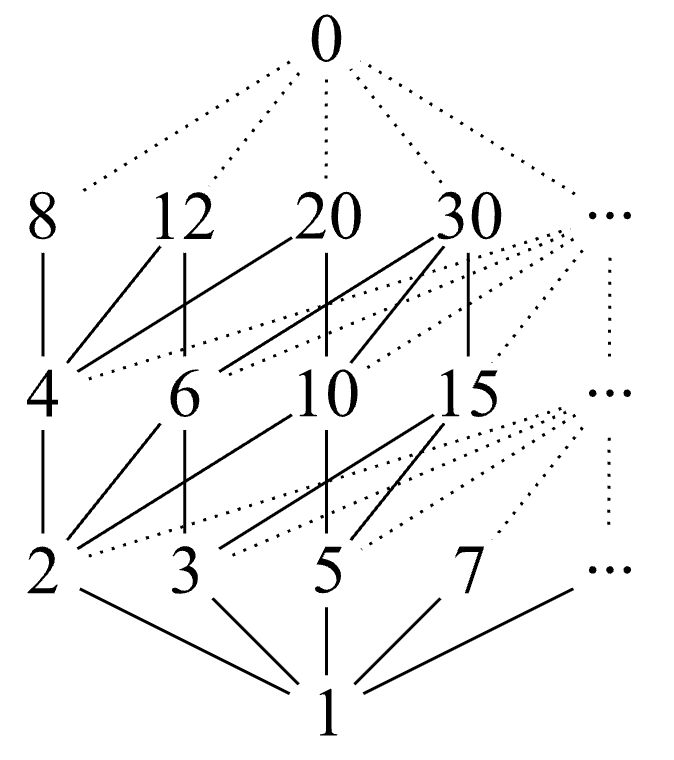
\includegraphics[width=100px]{fig/divisor_lattice.png}
\end{center}

The set $(\mathbb{N}, \preceq)$ forms a preorder. So,
what do products look like in $(\mathbb{N}, \preceq)$ considered 
as a category?
Let's consider the concrete instance of the product of $12$ 
and $16$. Let's consider the three possible interpretations of 
the product of $12$ and $16$ -- let's call it $X$ -- to understand what it means here:\marginnote{In what way 
is this behaving like an intersection?}
\begin{itemize}
  \item The graph-theoretic picture places the product in a diagram. 
  Suppose there is some natural number $Y$ such that $Y \preceq 12$ and $Y \preceq 16$.
  Then, the graphical depiction of the product $X$ 
  asserts the existence of a unique morphism $Y \to X$:
\begin{center}
  % https://tikzcd.yichuanshen.de/#N4Igdg9gJgpgziAXAbVABwnAlgFyxMJZABgBoAmAXVJADcBDAGwFcYkQBGckAX1PUy58hFOQrU6TVuw4A2XvxAZseAkQ6kOEhizaIQADQUCVw9aWLapekAE1eEmFADm8IqABmAJwgBbJADMNDgQSGIgjFhgNlAQODhOxiDefoHBoYhkIABGMGBQSAC0AcR8nj7+iEEgIUgaOXkFVaWKKZXhtZllyRVh6XU8lDxAA
\begin{tikzcd}
  & Y \arrow[d, dotted] \arrow[ldd, bend right] \arrow[rdd, bend left] &    \\
  & X \arrow[ld] \arrow[rd]                                            &    \\
12 &                                                                    & 16
\end{tikzcd}
\end{center}

  \item The order theoretic interpretation tells us that 
  $X$ is the greatest element that is less than both $12$
  and $16$ in the partial order -- i.e., it is the 
  greatest lower bound. In the case of this particular 
  partial order, this object has a special name: it is the 
  greatest common divisor.
\end{itemize}

Finally, similar to terminal objects, we say that a category $\calC$ \textbf{has
products} if for any two objects $A$ and $B$ in $\calC$ there exists an 
object $A \times B$ satisfying the universal property of products.

\section{Getting comfortable working with products}

Though we arrived at the definition of product through the \(\beta\)
and \(\eta\) laws for product types,
the universal property is taken as primary
as it is the one the generalizes to other type formers.
This property has three crucial parts.
Let \(\Gamma,A,B\) be objects and \(f : \Gamma \to A\)
and \(g : \Gamma \to B\). Then the following three facts hold:
\begin{enumerate}
\item There exists a morphism \(h : \Gamma \to P\).
\item The morphism \(h\) satisfies \(\pi_1 \circ h = f\) and \(\pi_2 \circ h = g\).
\item The morphism \(h\) is the \emph{unique} morphism satisfying property (2).
  This is made precise as follows:
  if any morphism \(h' : \Gamma \to P\) satisfies \(\pi_1 \circ h = f\)
  and \(\pi_2 \circ h = g\), then \(h' = h\).
\end{enumerate}
Taken together, these three bullet points say that
the special morphism \(h\) is \emph{defined by}
the property that \(\pi_1 \circ h = f\) and \(\pi_2 \circ h = g\).
A lot of proofs involving this universal property
perform equational reasoning
on the special morphisms \(h\).
Here is an example:
\begin{proposition}
  The following holds for all \(p : X \to Y\)
  and \(f : Y \to Z\) and \(g : Y \to W\)
  and products \((P,\pi_1,\pi_2)\) of \(Z\) and \(W\).
  \begin{align*}
  &(\text{the unique \(h\) such that \(\pi_1\circ h = f\) and \(\pi_2 \circ h = g\)})
  \circ p
  \\
  &= (\text{the unique \(h\) such that \(\pi_1 \circ h = f \circ p\)
  and \(\pi_2 \circ h = g \circ p\)})
  \end{align*}
\end{proposition}
Another example:
\begin{proposition}
  Let \((P,\pi_1,\pi_2)\) be a product of \(A\) and \(B\)
  in a category \(\calC\).
  Then
  \[
  (\text{the unique \(h\) such that \(\pi_1\circ h = \pi_1\)
  and \(\pi_2 \circ h = \pi_2\)})
  = \idt_{P}
  \]
\end{proposition}
It gets a little tiresome to write ``the unique \(h\) such that \(\pi_1 \circ h = f\)
and \(\pi_2 \circ h = g\)'' everywhere.
So category theorists use a convenient notational abbreviation
for this: the angle-bracketed expression \(\angled{f,g}\).\footnote{Note that 
this notational convention hides some data: in particular, 
it hides the codomain of $\langle f, g \rangle$. In practice this notational convention is quite useful 
because, as we will show later (in \cref{prop:prod-term}), products are 
isomorphic to each other, so hiding which particular choice of 
product object is utilized is prudent. Throughout category theory this 
sort of careful notation can be used (and confused!) to simplify arguments, but 
it's always important to know why a notational choice is valid.}
With this notation, the above propositions read as the following
algebraic identities:
\begin{align}
  \angled{\pi_1,\pi_2} &= \idt \\
  \angled{f,g}\circ p &= \angled{f\circ p, g \circ p}
\end{align}

These algebraic identities can then be used to prove more elaborate facts about
products.

\begin{proposition} \label{prop:products-commutative}
  Let \(\calC\) be a category with products.
  Then \(A\times B \cong B \times A\)
  for any objects \(A,B\) of \(\calC\).
\end{proposition}
\begin{proof}
  Since this is our first interesting proof we will give two arguments: one diagrammatic 
  that is from first-principles, and one that utilizes the algebraic identities we gave above.

  To show an isomorphism of objects we must find two morphisms:
  
  \begin{center}
   % https://tikzcd.yichuanshen.de/#N4Igdg9gJgpgziAXAbVABwnAlgFyxMJZABgBpiBdUkANwEMAbAVxiRAEEACAHW7wFt4nAEIgAvqXSZc+QigCM5KrUYs2wnnyyC4nduOUwoAc3hFQAMwBOEfkjIgcEJIpXNWiEBZDUARjDAoJABmYglLGztEVyd7PwCgxFDqBjp-BgAFaTwCNgYYCxwfNzVPYwMxIA
\begin{tikzcd}
  A \times B \arrow[r, "f", bend left] & B \times A \arrow[l, "g", bend left]
  \end{tikzcd}
  \end{center}
such that $g \circ f = \id_{A \times B}, f \circ g = \id_{B \times A}$.
We only have two ways of showing that two morphisms are equal to one 
another: by reading equations off commuting diagrams, or by showing that 
two morphisms satisfy the same universal property.
\end{proof}

Next, here is a theorem with a familiar shape, if one thinks of
products like the familiar notion of product of integers and terminal
objects as behaving like the product unit:

\begin{proposition}
  Let \(\calC\) be a category with products and a terminal object.
  Then \(1 \times A \cong A\) for any object \(A\) of \(\calC\).
\end{proposition}
\begin{proof}
  To show an isomorphism of objects, we need to show there exist
  morphisms $f$ and $g$:
  \begin{center}
  % https://tikzcd.yichuanshen.de/#N4Igdg9gJgpgziAXAbVABwnAlgFyxMJZABgBpiBdUkANwEMAbAVxiRAEEQBfU9TXfIRQBGclVqMWbYQAIAOnLwBbeDM5dxMKAHN4RUADMAThCVIyIHBCSiQAIxhgoSALQBmC-WatEIbSGoGOgcGAAV+PAI2IyxtAAscbl4QY1MbaitzagcnVw9A4JgwiMFo2ISAiW82A24KLiA
\begin{tikzcd}
  A \arrow[r, "g"', bend right] & 1 \times A \arrow[l, "f"', bend right]
  \end{tikzcd}
  \end{center}
  such that $f \circ g = \id_A$ and $g \circ f = \id_{1 \times A}$.
  Now pause: what morphisms $f$ and $g$ should we search for so that this is true? There's
  really only one choice, which we can see by looking at the types of these morphisms:
  \begin{center}
    % https://tikzcd.yichuanshen.de/#N4Igdg9gJgpgziAXAbVABwnAlgFyxMJZABgBpiBdUkANwEMAbAVxiRAEEQBfU9TXfIRQBGclVqMWbYQAIAOnLwBbeDM5dxMKAHN4RUADMAThCVIyIHBCSiQAIxhgoSALQBmC-WatEIBQzowbQYYeTkAoJCwo0DgmFIFJTocAAs4A2AsKC4AfXYFGMjWagCHBgAFfjwCNiMsbRScbl4QY1MbaitzagcnVw8SujLK7GqhEDqGpuovKV8FNCw87gouIA
\begin{tikzcd}
  A \arrow[r, "{\langle \langle \rangle,\mathsf{id}_A\rangle}"', bend right] & 1 \times A \arrow[l, "\pi_A"', bend right]
  \end{tikzcd}
  \end{center}

  So, we need to use the universal properties of product and terminal objects to
  construct these morphisms and show that they satisfy the necessary equations.
  This guides us to the following commuting diagram:\footnote{Note how we use
  the fact that $\mathbf{1}$ is terminal to fill in the leftmost leg of the diagram,
  and the fact that $1 \times A$ is a product to fill in $\pi_1$ and $\pi_A$.}

  \begin{center}
   % https://tikzcd.yichuanshen.de/#N4Igdg9gJgpgziAXAbVABwnAlgFyxMJZARgBoAGAXVJADcBDAGwFcYkQBBEAX1PU1z5CKcqQBM1Ok1btiPPiAzY8BImPGSGLNok7z+yoUTLFN0nSGIACADo28AW3hWu3STCgBzeEVAAzACcIByRREBwIJABmGi0ZXTtGejBPRhhbGySUtIyA5NSYUgyHehwACzg-YCwobgB9Dlz8tJAaRiwwCygIHBwPfRBA4OiaCKQyECSAIxhGAAUBFWFJmD8cVqltdjs0LDq5Xn8gkMQY8MjEdU34kB291wUhk7CxxAmZsCgkAFoosLiLIlmuk7Hlsmw2vQZvNFkZdAEsJ4yutDoNjqFRhcrh8vqd-uZtjYSuVKtVag0eJRuEA
\begin{tikzcd}
  & A \arrow[d, "{\langle \langle \rangle, \mathsf{id}_A \rangle}", dotted] \arrow[ldd, "\langle \rangle"', bend right] \arrow[rdd, "\mathsf{id}_A", bend left] &   \\
  & 1 \times A \arrow[ld, "\pi_1"] \arrow[rd, "\pi_A"]                                                                                                          &   \\
1 &                                                                                                                                                             & A
\end{tikzcd}
  \end{center}

  Reading equations off this diagram, we have:
  \begin{align}
    \id_A = \pi_A \circ \langle \langle \rangle, \id_A \rangle
  \end{align}
  This is one half of our required isomorphism.

\end{proof}

\begin{definition}[Ternary product]
  Let \(A,B,C\) be objects of a category \(\calC\).
  A \emph{ternary product} of \(A,B,C\)
  is a tuple \((P,\pi_A,\pi_B,\pi_C)\)
  where \(\pi_A : P\to A\) and \(\pi_B : P \to B\)
  and \(\pi_C : P \to C\)
  and the following universal property holds:
  for any object \(\Gamma\)
  and morphisms \(f : \Gamma \to A\)
  and \(g : \Gamma \to B\) and \(h : \Gamma \to C\),
  there exists a unique morphism \(k : \Gamma \to P\)
  such that \(\pi_A \circ k = f\)
  and \(\pi_B \circ k = g\) and \(\pi_C \circ k = h\).
\end{definition}

\begin{proposition}
  Let \(A,B,C\) be objects in a category \(\calC\) with products.
  The tuple \((A\times (B\times C), \pi_A, \pi_B \circ \pi_{B\times C}, \pi_C \circ \pi_{B\times C})\)
  is a ternary product of \(A,B,C\).
\end{proposition}

\begin{definition}[Finite products] \label{def:finite-products}
  A category has \textbf{finite products}
  if it has products~(Def~\ref{def:product}) and a terminal object~(Def~\ref{def:terminal-object}).
\end{definition}

\section{Initial objects \& duality}
The categorical perspective can push you towards new ideas you may not have
thought of. Here's an example of this: given a category $\calC$, thought of as a
graph, one can do a natural thing: \emph{flip the direction of all arrows in the
opposite direction}. This new category is called the \textbf{opposite category},
and is written $\calC^\text{op}$.
Relationships between properties of $\calC$ and properties of its opposite 
category $\calC^\text{op}$ are broadly referred to as \textbf{dualities}.

Dualities can be a source of free ideas. For instance, let's consider the
dual notion of a terminal object where we flip the direction of the arrows:

\begin{definition}[Initial object] 
  \sloppy
  Let $I$ be an object in a category $\calC$. 
  An object $I$ in $\calC$ is called an initial object
  if, for every other object $A$ in $\calC$ there exists a unique 
  morphism $I \xrightarrow{} C$. Graphically,

  \begin{center}
% https://tikzcd.yichuanshen.de/#N4Igdg9gJgpgziAXAbVABwnAlgFyxMJZABgBpiBdUkANwEMAbAVxiRAEEQBfU9TXfIRQBGclVqMWbACrdxMKAHN4RUADMAThAC2SMiBwQkokAyxhWiEHAhmoIagzoAjGAwAK-PATYMYanAcJZksQAB0wmAAPLDgcOABCOS4gA
\begin{tikzcd}
  I \arrow[r, "\exists!"] & A
  \end{tikzcd}
\end{center}
\end{definition}

Note that an object that is terminal in $\calC$ must be initial 
in $\calC^\text{op}$ and vice versa: this is what characterizes 
the terminal object as dual to the initial object. 

Now that we have a ``free'' universal construction, it might be 
natural to ask: \emph{is there an interesting type that this 
special initial object corresponds to}? Indeed there is: the 
initial object corresponds to the $\plVoid$ type that 
has no inhabitants. It has the following typing rules:

\begin{mathpar}
\inferrule{M : \plVoid}{\Gamma \vdash \texttt{absurd}~M : A}
\end{mathpar}

Intuitively, the $\plVoid$ type represents logical absurdity or 
``invalid program state''.
Some programming languages have a construct for working with 
void types and absurdity: Haskell has the void, which is 
eliminated with \texttt{absurd}.



\section{Products as Terminal Objects ($*$)}
\marginnote{Sections marked with $*$ are optional and won't be covered in class.}
\label{sec:products-as-terminal-objects}

The diagrammatic form suggests a
a order-based intuition for products:
the product \((P,p,q)\) is
in some sense the ``largest''
tuple of that shape,
with its universal property
showing that any other tuple of the same shape is
``less than or equal'' to it by virtue of the existence of
the dashed morphism.

\begin{definition}[Category of rooted spans]
  \sloppy
  Let \(A\) and \(B\) be objects of a category \(\calC\).
The category of \emph{spans in \(\calC\) rooted at \(A\) and \(B\)},
written \(\mathsf{Span}_\calC(A,B)\),
is the category whose
\begin{itemize}
  \item Objects are tuples \((X,f,g)\)
    where \(X\) is an object of \(\calC\),
    \(f : X \to A\), and \(g : X \to B\).
    Pictorially:
    \[% https://tikzcd.yichuanshen.de/#N4Igdg9gJgpgziAXAbVABwnAlgFyxMJZABgBoBGAXVJADcBDAGwFcYkQANEAX1PU1z5CKcqWLU6TVuwCCPPiAzY8BIqIBMEhizaIQAIR4SYUAObwioAGYAnCAFskZEDghJ1NbdL2mQNRvQARjCMAAoCKsIgNlimABY48tZ2jojOrkiikjrsVkbcQA
\begin{tikzcd}
                                   & A \\
X \arrow[rd, "g"'] \arrow[ru, "f"] &   \\
                                   & B
\end{tikzcd}\]
  \item A morphism is a tuple
    \(((X,f,g),\alpha,(X',f',g'))\)
    where \((X,f,g)\) and  \((X',f',g')\)
    are objects and \(\alpha : X \to X'\)
    is a morphism of \(\calC\)
    such that \(f' \circ \alpha = f\)
    and \(g' \circ \alpha = g\).
    Pictorially:
    \[% https://tikzcd.yichuanshen.de/#N4Igdg9gJgpgziAXAbVABwnAlgFyxMJZABgBoBGAXVJADcBDAGwFcYkQANEAX1PU1z5CKAEyli1Ok1bsAgjz4gM2PASJiRkhizaIQAIQX8VQouQpbpuzgHIekmFADm8IqABmAJwgBbJGRAcCCQxKR12JxAaRnoAIxhGAAUBVWEQTywnAAscKJB4sCgkAFoAZmJeD28-RACgpHMwmT13PIKixHLKkC9fJFKaesRG7Waeu2i4hOSTNT0M7Nzu3pqBwODEUNHrJztl6v9BjbXt9gAdM6Y0LPp7biA
\begin{tikzcd}
                                                                                &                                       & A \\
X \arrow[rrd, "g"', bend right] \arrow[rru, "f", bend left] \arrow[r, "\alpha"] & X' \arrow[ru, "f'"'] \arrow[rd, "g'"] &   \\
                                                                                &                                       & B
\end{tikzcd}\]

\item Composition is defined by
  \begin{align}
    &((X',f',g'),\alpha',(X'',f'',g''))\circ ((X,f,g),\alpha,(X',f',g'))\\
    &= ((X,f,g),\alpha'\circ \alpha,(X'',f'',g'')).
  \end{align}
  Pictorially:
  \begin{equation}
    % https://tikzcd.yichuanshen.de/#N4Igdg9gJgpgziAXAbVABwnAlgFyxMJZAJgBoAGAXVJADcBDAGwFcYkQBBEAX1PU1z5CKMsWp0mrdgCEefEBmx4CRMgEZxDFm0QgAGgHIDc-kqFE1pDTS1TdhkwoHLhyclc2Sd+493EwoAHN4IlAAMwAnCABbJDIQHAgkdwltdjCjR0iYuJpEpEtUuxBAzJpGegAjGEYABWdzXQisQIALHCyo2MQAZjykxHjbbwAdEaY0VvpfeWzuvoSBlOH04xpqsChk3nCupAX8xEKNrcRlr3ZSkHKqmvqzFSaW9s6cxAAWfuT1mE3987SujCr26n0WBR+f0QAFoegDioFriAKtU6g1HiBmm0OjsQHMkGDDgsVroxhMpjxKNwgA
\begin{tikzcd}
                                                                                 &                                                            & A                                      \\
X' \arrow[rru, "f", bend left] \arrow[rrd, "g"', bend right] \arrow[r, "\alpha"] & X' \arrow[r, "\alpha'"] \arrow[ru, "f'"] \arrow[rd, "g'"'] & X'' \arrow[u, "f''"] \arrow[d, "g''"'] \\
                                                                                 &                                                            & B
\end{tikzcd}
  \end{equation}

  \item The identity morphism at \((X,f,g)\) is \(((X,f,g),\idt_{X},(X,f,g))\).
\end{itemize}
The associativity and identity laws in \(\mathsf{Span}_\calC(A,B)\)
are inherited from the corresponding laws for in \(\calC\).
\end{definition}

This perhaps tortured-looking category serves a valuable purpose:
it makes precise the sense in which a product \((P,p,q)\)
is the ``largest'' among such tuples.

\begin{proposition}
  \label{prop:prod-term}
  Let \(A\) and \(B\) be objects of a category \(\calC\).
  A tuple \((P,p,q)\) is a product of \(A\) and \(B\)
  if and only if it is a terminal object of \(\mathsf{Span}_\calC(A,B)\).
\end{proposition}

To unpack what this is saying, from the perspective of categories as metalanguages:
a product for \(A\) and \(B\) in the metalanguage embodied
by \(\calC\) is a unit type for the metalanguage
embodied by \(\mathsf{Span}_\calC(A,B)\).
Some of the power of category theory can be seen here:
\begin{itemize}
\item Constructions on categories can be used to quickly build
  nontrivial ``metalanguages'' from old.
  (What would \(\mathsf{Span}_\calC(A,B)\) even look like as a traditional language?)
\item Category theory ``eats itself'': the categorical notion of terminal object
  sheds light on the categorical notion of product, if one knows to look at
  the right category.
\end{itemize}
To illustrate the benefits of this perspective,
we get a proof that products are suitably unique
just like terminal objects are, simply because they \emph{are terminal objects}:
\begin{proposition}
  Products are unique up to unique isomorphism.
\end{proposition}
\begin{proof}
  Products are terminal objects,
  and terminal objects are unique up to unique isomorphism.\footnote{Phew! What a nice short proof!}
\end{proof}




\chapter{PL Interlude: First-order STLC}

Recall the language \textsc{Calc} from \Cref{sec:semantics-of-programs}.
\begin{gather}
  \begin{aligned}
  M,N &::= \pllet{x}{M}{N} \mid x \mid \plunit{} \mid \plpair{M}{N} \mid \plfst{M} \mid \plsnd{M} \\
  A,B &::= A \times B \mid \plUnit
  \end{aligned}
  \tag{\textsc{Calc}}
  \label{lang:calc}
\end{gather}
We have been slowly and informally building a dictionary between
syntactic operations and categorical ones.
First there is the way that each judgment is interpreted:
\begin{itemize}
\item Types are objects
\item Contexts are products
\item Terms are morphisms
\item Equations are equalities of morphisms
\end{itemize}
Then there is the way each term former is interpreted,
in terms of the canonical operations on products and terminal objects:
\begin{itemize}
\item Fst, snd, tupling + laws
\item Unit + laws
\end{itemize}
Finally there is the way that structural operations are interpreted:
\begin{itemize}
\item Variable lookup is projection
\item Let-binding is (multi)composition
\end{itemize}
Taken together, these constructions establish the following:
\begin{theorem} \label{thm:calc-products}
  \textsc{Calc} can be interpreted in any category with finite products~(\cref{def:finite-products}).
\end{theorem}
\begin{proof}
  Let \(\calC\) be a category with products and a terminal object.
  We will build an interpretation function \(\llbr{-}\)
  that maps each of the judgments of \textsc{Calc}
  into \(\calC\):
  \begin{itemize}
  \item Types \(A\) will become \(\llbr{A}\) of \(\calC\).
  \item Contexts \(\Gamma\) will become objects \(\llbr{\Gamma}\) of \(\calC\).
  \item Derivations of \(\Gamma \vdash M : A\) will become
    morphisms \(\llbr{\Gamma} \xlongrightarrow{\llbr{M}} \llbr{A}\).
  \item Derivations of \(\Gamma \vdash M \equiv N : A\) will become
    equalities:
    \[% https://tikzcd.yichuanshen.de/#N4Igdg9gJgpgziAXAbVABwnAlgFyxMJZABgBoBGAXVJADcBDAGwFcYkQAdDxxgIwCdgXAOL0AtmPoBfEFNLpMufIRQAmCtTpNW7LjwHAAgjLkLseAkXKlimhizaIQs+SAznlV0qrvbHzqU0YKABzeCJQADN+CDEkMhAcCCRrEF4YMCgkAGYE+x0nPT5BAFkTV2jY+JoklJp0zKQAWlyafP8igwA5GRpGenTGAAVFCxUQfiwQgAscFyiYuMR1ROTEbL6sMH9IbZAaaZh6LKddthr6LEZ2M-2QfsGRj0snLexYO-b2AD8uGJx6DgYLwIAAPYAATmIUiEHAAFABeLgAShMlCkQA
\begin{tikzcd}
                                                                                    & {} \arrow[dd, "~\rotatebox{90}{\(=\)}", phantom] &          \\
\llbr{\Gamma} \arrow[rr, "\llbr{M}", bend left] \arrow[rr, "\llbr{N}"', bend right] &                                                  & \llbr{A} \\
                                                                                    & {}                                               &
\end{tikzcd}\]
  \end{itemize}
  Each of these will be defined by induction.\footnote{
  Warning: this is going to take a while.
  }

  First, let us interpret \textsc{Calc} types.
  \begin{align}
    \llbr{\plUnit} &= 1 \\
    \llbr{A \pltimes B} &= \llbr{A} \times \llbr{B}
  \end{align}
  These equations look just like
  (\ref{eqn:calc-types-in-finset}), the interpretation
  of types given in Section~\ref{sec:calc-in-finset}.
  But their meaning is very different.
  Whereas before the operator \(\times\) was used
  to denote the Cartesian product of finite sets,
  here it denotes the categorical
  product of the objects \(\llbr{A}\) and \(\llbr{B}\)
  of an arbitrary category \(\calC\).
  Similarly, \(1\) denotes the terminal object in \(\calC\),
  not the singleton set \(\{\star\}\).

  The interpretation of \textsc{Calc} contexts is similarly straightforward.
  The empty context is interpreted as the terminal object
  and context extension is interpreted via product.
  \begin{align}
    \llbr{\ctxemp} &= 1 \\
    \llbr{\Gamma, x\ofty A} &= \llbr{\Gamma} \times \llbr{A}
  \end{align}

  Next up we have the interpretation of typing derivations.
  This is where things start getting interesting.
  We have one case per typing rule. As a warm-up,
  here is the interpretation of the typing rule for \(\plunit\).
  \begin{align}
    \llbr{
      \frac
        {~}
        {\Gamma \vdash \plunit : \plUnit}
    }
    = \angled{}_{\llbr{\Gamma}}
  \end{align}
  In words: the interpretation of \(\plunit\)
  with respect to typing context \(\Gamma\)
  is the unique morphism \(\angled{}_{\llbr{\Gamma}}\)
  from \(\llbr{\Gamma}\) to \(\llbr{\plunit}\),
  guaranteed to exist because \(\llbr{\plunit}\)
  is a terminal object of \(\calC\).

  The interpretation of \(\plunit\) is special because its typing rule has no premises.
  More generally, the interpretations of the other typing rules
  will rely inductively on interpretations of premises.
  For instance, here is the interpretation of the typing rule for \(\plfst{M}\).
  \begin{align}
    \llbr{
      \displaystyle\frac
        {\displaystyle\frac{\vdots}{{{{\Gamma \vdash M : A \pltimes B}}}}}
        {\Gamma \vdash \plfst{M} : A}
    }
    = \pi_1 \circ \llbr{\frac{\vdots}{\Gamma \vdash M : A \pltimes B}}
  \end{align}
  \footnote{\todo: Really wish I knew how to fix the spacing here.}
  In words: to interpret a typing derivation for \(\plfst{M}\)
  as shown, first interpret the subderivation
  establishing \(\Gamma \vdash M : A \pltimes B\)
  to obtain a morphism \(\llbr{\Gamma} \xrightarrow{\llbr{M}} \llbr{A\pltimes B}\),
  and then compose this morphism with the projection
  \(\llbr{A\pltimes B} \xrightarrow{\pi_1} \llbr{A}\),
  guaranteed to exist because \(\llbr{A \pltimes B}\)
  is a product of \(\llbr{A}\) and \(\llbr{B}\).

  The typing rule for \(\plsnd{M}\) is interpreted analogously.
  \begin{align}
    \llbr{
      \displaystyle\frac
        {\displaystyle\frac{\vdots}{{{{\Gamma \vdash M : A \pltimes B}}}}}
        {\Gamma \vdash \plsnd{M} : B}
    }
    = \pi_2 \circ \llbr{\frac{\vdots}{\Gamma \vdash M : A \pltimes B}}
  \end{align}

  The pair formation rule is interpreted using the universal property of product.
  \begin{align}
    \llbr{
      \displaystyle\frac
        {\displaystyle\frac{\vdots}{{{{\Gamma \vdash M : A}}}}
          \qquad
         \displaystyle\frac{\vdots}{{{{\Gamma \vdash N : B}}}}
        }
        {\Gamma \vdash \plpair{M}{N} : A \pltimes B}
    }
    = \left\langle
      \llbr{\frac{\vdots}{\Gamma \vdash M: A}}
      ,
      \llbr{\frac{\vdots}{\Gamma \vdash N: B}}
    \right\rangle
  \end{align}

  Finally we have the typing rules for variables and let-bindings.
  We have saved these rules for last because they highlight some
  interesting points regarding the categorical interpretation
  of operations on the typing context \(\Gamma\).

  First let us see how to interpret variables.
  Because typing contexts \(\Gamma\) are interpreted as iterated products,
  variables are interpreted as projections:
  \begin{align}
    \llbr{
      \frac{(x:A)\in\Gamma}{\Gamma \vdash x : A}
    }
    = \pi_x
  \end{align}
  In words: \(\pi_x\) is the canonical projection
  \(\llbr{\Gamma} \to \llbr{A}\)
  that extracts the
  ``\(x\)th component'' out of
  the iterated product used to define \(\llbr{\Gamma}\).

  You may find this intepretation of variables unsatisfying:
  what exactly is this ``canonical'' projection,
  and what does it mean to take the ``\(x\)th component''?
  Here is one way to make this precise.
  The trick is to reformulate the typing rule for variables
  in terms of two more elementary rules:
  \begin{mathpar}
    \inferrule*[right=Hit]
      {~}
      {\Gamma,x\ofty A \vdash x : A}
    \and
    \inferrule*[right=Miss]
      {\Gamma \vdash x : A}
      {\Gamma,y\ofty B \vdash x : A}
  \end{mathpar}
  Together these rules can be thought of as definign
  a procedure for checking whether a given binding \((x:A)\)
  lives in a given typing context \(\Gamma\).
  The rule \textsc{Hit} covers the case where \((x:A)\)
  matches the variable right at the end of the typing context.
  The rule \textsc{Miss} covers the case where
  it doesn't and one has to keep looking further into \(\Gamma\).

  This reformulation of the variable rule allows for a precise
  definition of the handwavy \(\pi_x\).
  \begin{align}
    \llbr{
      \frac
        {~}
        {\Gamma,x\ofty A \vdash x : A}
        ~(\textsc{Hit})
    }
    &= \pi_2
    \\
    \llbr{
      \frac
        {\displaystyle\frac{\vdots}{\Gamma \vdash x : A}}
        {\Gamma,y\ofty B \vdash x : A}
        ~(\textsc{Miss})
    }
    &=
    \llbr{
      \frac{\vdots}{\Gamma \vdash x : A}
    }
    \circ \pi_1
  \end{align}
  Using these two rules,
  we can see that \(\pi_x\) is actually a composite consisting of a string of \(\pi_1\)s followed by a \(\pi_2\),
  with the length of this string depending on where \(x\) appears in \(\Gamma\). For instance,
  \begin{align}
    &\llbr{\frac{\vdots}{x\ofty A, y\ofty B, z\ofty C \vdash x : A}} \\
    &=
    \llbr{\frac{\vdots}{x\ofty A, y\ofty B \vdash x : A}} \circ \pi_1 \\
    &=
    \llbr{\frac{\vdots}{x\ofty A \vdash x : A}} \circ \pi_1 \circ \pi_1 \\
    &=
    \pi_2 \circ \pi_1 \circ \pi_1.
  \end{align}
  Note that there are two \(\pi_1\)s in this composite. This corresponds to the fact that
  the de Bruijn index of \(x\) in the context \(x\ofty A,y\ofty B,z\ofty C\) is two.\footnote{%
    You are now a third of the way through
  the proof of Theorem~\ref{thm:calc-products}.}


  With variables out of the way, let us now turn to let-bindings.
  These also illustrate an interesting interaction
  between operations on the typing context and categorical products.
  \begin{align*}
    &\llbr{
      \frac
      {
        \displaystyle\frac{\vdots}{\Gamma\vdash M : A}
        \qquad
        \displaystyle\frac{\vdots}{\Gamma,x\ofty A\vdash N : B}
      }
      {\Gamma\vdash \pllet{x}{M}{N} : B}
    }
    \\
    &=
    \llbr{\frac{\vdots}{\Gamma,x\ofty A \vdash N : B}}
    \circ
    \left\langle
    \idt_{\llbr{\Gamma}}
    ,
    \llbr{\frac{\vdots}{\Gamma\vdash M : A}}
    \right\rangle
  \end{align*}
  Let's break this down a bit.
  By induction, we have that
  \(M\) denotes a morphism \(\llbr{\Gamma} \to \llbr{A}\)
  and \(N\) denotes a morphism \(\llbr{\Gamma,x\ofty A} = \llbr{\Gamma}\times\llbr{A} \to \llbr{B}\).
  The interpretation of \(\pllet{x}{M}{N}\)
  composes these together. The twist is that,
  because the variables in \(\Gamma\) are shared between \(M\)
  and \(N\), the object \(\llbr{\Gamma}\)
  plumbed around as well.
  This is accomplished by the morphism
  \(
    \left\langle
    \idt_{\llbr{\Gamma}}
    ,
    \llbr{\Gamma\vdash M : A}
    \right\rangle\)
    guaranteed to exist
    by the universal property of products.

  In practice, it's fairly laborious to write down
  the interpretation function explicitly as a function
  on derivations as we have done above.
  So people tend to shorten the more verbose
  \(\llbr{\dfrac{\vdots}{\Gamma\vdash M : A}}\)
  to just
  \(\llbr{M}\). Written this way, the foregoing discussion
  can be summarized in terms of the following
  equations.
  \begin{align*}
    \llbr{\plunit} &= \angled{} \\
    \llbr{\plfst{M}} &= \pi_1 \circ \llbr{M} \\
    \llbr{\plsnd{M}} &= \pi_2 \circ \llbr{M} \\
    \llbr{\plpair{M}{N}} &= \angled{\llbr{M},\llbr{N}} \\
    \llbr{x} &= \pi_x \\
    \llbr{\pllet{x}{M}{N}} &=
      \llbr{N} \circ \angled{\idt_{\llbr{\Gamma}},\llbr{M}}
  \end{align*}
  In some cases it is desirable
  to have an interpretation function that operates
  directly on terms,
  rather than on derivations,
  as derivations can contain extraneous information
  not present in a term.
  In these cases a tricky issue comes up:
  for \(\llbr{-}\) to be a functions on terms,
  it must be the case that
  the denotation of a term does not depend on
  the precise way in which it is proved to be well-typed.
  Checking this \emph{coherence condition}
  involves showing that, for any term \(M\),
  the denotations of all typing derivations
  for \(M\) are equal~\citep{reynolds1991coherence}.
  In our case \textsc{Calc} satisfies the property that every term has at most one typing derivation
  when each bound variable is annotated with its type,
  so we won't worry too much about this.

  We have now seen how to interpret the types,
  typing contexts, and typing derivations of \textsc{Calc}.
  Only one task remains: interpret derivations of
  \(\Gamma \vdash M \equiv N : A\).
  There are five groups of rules to interpret.
  \begin{enumerate}
  \item First there are the rules stating that \(\equiv\)
    is an equivalence relation on well-typed terms.
    \begin{mathpar}
      \inferrule*[right=Refl]
        {\Gamma \vdash M : A}
        {\Gamma \vdash M \equiv M : A}
      \and
      \inferrule*[right=Sym]
        {\Gamma \vdash M \equiv N : A}
        {\Gamma \vdash N \equiv M : A}
      \and
      \inferrule*[right=Trans]
        {\Gamma \vdash M \equiv N : A
          \\
         \Gamma \vdash N \equiv O : A
        }
        {\Gamma \vdash M \equiv O : A}
    \end{mathpar}
  \item Next there are the \emph{congruence rules},
    so called because they state that \(\equiv\)
    is a congruence for each of the \textsc{Calc} term formers.\footnote{%
     In general, an equivalence relation \(\sim\) on a set \(X\)
     is a \emph{congruence} with respect to a function
     \(f : X \to X\) if \(x \sim x'\) implies \(f(x) \sim f(x')\).}
    \begin{mathpar}
      \inferrule*[right=Cong-Pair]
        {\Gamma \vdash M \equiv M' : A
          \\
         \Gamma \vdash N \equiv N' : B
        }
        {\Gamma \vdash \plpair{M}{N} \equiv \plpair{M'}{N'} : A \pltimes B}
      \and
      \inferrule*[right=Cong-Fst]
        {\Gamma \vdash M \equiv M' : A \pltimes B
        }
        {\Gamma \vdash \plfst{M} \equiv \plfst{M'} : A}
      \and
      \inferrule*[right=Cong-Snd]
        {\Gamma \vdash M \equiv M' : A \pltimes B
        }
        {\Gamma \vdash \plsnd{M} \equiv \plsnd{M'} : A}
      \and
      \inferrule*[right=Cong-Let]
        {\Gamma \vdash M \equiv M' : A
          \\
        \Gamma, x\ofty A \vdash N \equiv N' : B
        }
        {\Gamma \vdash (\pllet{x}{M}{N}) \equiv (\pllet{x}{M'}{N'}) : B}
    \end{mathpar}
  \item Then there are the \emph{\(\beta\) laws}
    that describe what happens when one applies an introduction
    form for a given type former followed by an elimination form.
    \begin{mathpar}
      \inferrule*[right=\(\beta^{\pltimes}_1\)]
        {\Gamma \vdash M : A
          \\
          \Gamma \vdash N : B
        }
        {\Gamma \vdash \plfst{\plpair{M}{N}} \equiv M : A}
    \and
      \inferrule*[right=\(\beta^{\pltimes}_2\)]
        {\Gamma \vdash M : A
          \\
          \Gamma \vdash N : B
        }
        {\Gamma \vdash \plfst{\plpair{M}{N}} \equiv N : B}
    \end{mathpar}
  \item Then there are the \emph{\(\eta\) laws}
    that describe what happens when one applies an elimination form
    followed by an introduction form.
    \begin{mathpar}
      \inferrule*[right=\(\eta^{\pltimes}\)]
        {\Gamma \vdash M : A \pltimes B}
        {\Gamma \vdash \plpair{\plfst{M}}{\plsnd{M}} \equiv M : A \pltimes B}
    \and
      \inferrule*[right=\(\eta^{\plUnit}\)]
        {\Gamma \vdash M : \plUnit
        }
        {\Gamma \vdash \plunit \equiv M : \plUnit}
    \end{mathpar}
  \item Last but not least, there is the law
    that let-binding is equivalent to substitution.
    \begin{mathpar}
      \inferrule*[right=Let-Sub]
        {\Gamma \vdash M : A
          \\
        \Gamma, x\ofty A \vdash N : B
        }
        {\Gamma \vdash (\pllet{x}{M}{N}) \equiv N[M/x] : B}
    \end{mathpar}
  \end{enumerate}
  Let us tackle each of these groups one by one.

  These rules in group (1) are easy to interpret:
    they correspond directly to the reflexivity,
    symmetry, and transitivity of equality of morphisms.
    For instance,
    the \textsc{Sym} rule holds because,
    if \(\llbr{M} = \llbr{N}\) for some well-typed terms \(M\) and \(N\),
    then also \(\llbr{N} = \llbr{M}\).\footnote{%
    The stickler may wonder how we know that \(M\)
    and \(N\) are well-typed here, since all we have
    in the premise of \textsc{Sym}
    is that \(M\equiv N\).
    It turns out that
    \(\equiv\) satisfies the following property:
    if \(\Gamma \vdash M \equiv N : A\),
    then \(\Gamma \vdash M : A\)
    and \(\Gamma\vdash N : A\).
    This fact can be established by induction on derivations
    of \(\Gamma \vdash M \equiv N : A\),
    and we won't belabor it.
    A slicker way of maintaining this well-typedness invariant
    throughout the definition of \(\equiv\)
    is to make well-typedness a \emph{presupposition}
    of the judgment \(\Gamma \vdash M \equiv N : A\)~\citep{martin1996meanings}.
    }

  The rules in group (2) are also relatively easy.
  In each case the proof boils down to showing that
  a given operation on morphisms respects equality.
  For instance, the rule \textsc{Cong-Pair}
  boils down to the following true statement:
  if \(\llbr{M} = \llbr{M'}\)
  and \(\llbr{N} = \llbr{N'}\)
  then \(\angled{\llbr{M},\llbr{M'}} = \angled{\llbr{N},\llbr{N'}}\).
  The other cases are similarly straightforward.

  The rules in group (3) follow from the definition of categorical product.
  The law \(\beta^{\pltimes}_1\) boils down to showing that
  \(\pi_1 \circ \angled{\llbr{M},\llbr{N}} = \llbr{M}\).
  The law \(\beta^{\pltimes}_2\) is analogous.

  The rules in group (4) follow from the definitions of categorical product
  and terminal object. First, the law \(\eta^{\plUnit}\)
  follows from the fact that any two morphisms into a terminal object are equal.
  The law \(\eta^{\pltimes}\) boils down to showing
  that, for any morphism \(\llbr{M} : \llbr{\Gamma} \to \llbr{A} \times \llbr{B}\),
  it is the case that \(\llbr{M} = \angled{\pi_1\circ \llbr{M}, \pi_2\circ\llbr{M}}\).
  This follows from a uniqueness argument.
  By definition, \(\angled{\pi_1\circ \llbr{M}, \pi_2\circ\llbr{M}}\)
  is the unique morphism \(f\) satisfying \(\pi_1\circ f = \pi_1 \circ \llbr{M}\)
  and \(\pi_2\circ f = \pi_2 \circ \llbr{N}\). But \(\llbr{M}\)
  satisfies this same property. Hence \(\llbr{M} = f = \angled{\pi_1\circ\llbr{M}, \pi_2\circ\llbr{M}}\).

  All that's left is \textsc{Let-Sub}---the rule stating that let-binding is equivalent to substitution.
  Validating this rule boils down to showing the following:
  \begin{lemma} \label{lem:let-is-subst}
    For all contexts \(\Gamma\), types \(A\),
    and terms \(M\) and \(N\)
    such that \(\Gamma \vdash M : A\)
    and \(\Gamma,x\ofty A \vdash N : B\),
    it holds that
    \(\llbr{N[M/x]} = \llbr{N} \circ \angled{\idt_{\llbr{\Gamma}},\llbr{M}}\).
  \end{lemma}
  This lemma essentially relates
  the syntactic operation of substituting
  of \(M\) into \(N\)
  with the semantic operation
  of composing the morphism \(\llbr{N}\) with \(\angled{\idt_{\llbr{\Gamma}},\llbr{M}}\).

  A natural proof strategy to try here is to proceed by induction on (a typing derivation for) \(N\),
  as the substitution operation \(N[M/x]\) is defined recursively on it.
  But this approach runs into a problem: the induction hypothesis one gets is not
  strong enough.
  The problematic case is when \(N = (\pllet{x'}{N_1}{N_2})\).
  In this case, we have that
  \begin{enumerate}
  \item \(\Gamma,x\ofty A \vdash N_1 : A'\) for some type \(A'\)
  \item \(\Gamma,x\ofty A,x'\ofty A' \vdash N_2 : B\)
  \end{enumerate}
  and the goal is to show that
  \begin{equation}
    \llbr{(\pllet{x'}{N_1}{N_2})[M/x]} = \llbr{\pllet{x'}{N_1}{N_2}} \circ \angled{\idt_{\llbr{\Gamma}},\llbr{M}}.
  \end{equation}
  By the definition of substitution, we have that
  \[
  (\pllet{x'}{N_1}{N_2})[M/x] = (\pllet{x'}{N_1[M/x]}{N_2[M/x]}).
  \]
  At first glance, this equation looks awfully provable from the above assumptions,\footnote{%
    You are now two thirds of the way through the proof of Theorem~\ref{thm:calc-products}.}
  by applying the induction hypothesis to
  the terms \(N_1[M/x]\) and \(N_2[M/x]\) and then performing some algebraic manipulations.
  But a closer look will reveal that \(N_2[M/x]\) actually does not fit the shape required
  for the induction hypothesis to apply.
  This is because our induction hypothesis only applies to substitutions of \(M\)
  into terms well-typed in context \(\Gamma,x\ofty A\).
  On the other hand, \(N_2[M/x]\) is a substitution
  of \(\Gamma \vdash M : A\) into \(\Gamma,x\ofty A,{\color{red}x'\ofty A'} \vdash N_2 : B\).
  This extra red entry in the typing context does not match the shape of our induction hypothesis.

  What has happened here is that the statement of Lemma~\ref{lem:let-is-subst}
  applies only to terms of the form \(N[M/x]\) where \(x\) is the right-most variable
  in the typing context used to type \(N\). But while performing the substitution \(N[M/x]\),
  we will recursively substitute \(M\) into subterms where \(x\) is \emph{not} the right-most variable
  anymore, due to the presence of let-bindings.
  Thus there is a mismatch between the recursive structure of the substitution function
  and the shape of our inductive argument.

  We can remedy this by strengthening Lemma~\ref{lem:let-is-subst}
  to the following statement, which applies to terms \(N[M/x]\) where \(x\) may occur anywhere in the context.
  \begin{lemma} \label{lem:let-is-sub-stronger}
    For all contexts \(\Gamma\) and \(\Delta\), types \(A\),
    and terms \(M\) and \(N\)
    such that \(\Gamma \vdash M : A\)
    and \(\Gamma,x\ofty A,\Delta \vdash N : B\),
    it holds that
    \(\llbr{N[M/x]} = \llbr{N} \circ \angled{\pi_{\llbr{\Gamma}},\llbr{M} \circ \pi_{\llbr{\Gamma}},\pi_{\llbr{\Delta}}}\).
  \end{lemma}
  The statement of Lemma~\ref{lem:let-is-sub-stronger} requires some clarification.

  First, it involves morphisms
   \(\llbr{\Gamma,\Delta} \xrightarrow{\pi_{\llbr{\Gamma}}} \llbr{\Gamma} \)
  and
   \(\llbr{\Gamma,\Delta} \xrightarrow{\pi_{\llbr{\Delta}}} \llbr{\Delta}\).
  These morphisms are defined by the following fact, which can be proved
  by induction on \(\Delta\): for all \(\Gamma\) and \(\Delta\)
  it holds that \(\llbr{\Gamma,\Delta}\) is a product of \(\llbr{\Gamma}\) and \(\llbr{\Delta}\).
  The morphisms \(\pi_{\llbr{\Gamma}}\) and \(\pi_{\llbr{\Delta}}\) are the projections
  out of this product.

  Second, we have used a ternary angle-bracket operator
  to form the morphism \(\angled{\pi_{\llbr{\Gamma}},\llbr{M}\circ\pi_{\llbr{\Gamma}},\pi_{\llbr{\Delta}}}\).
  This notation is justified by the following fact, which also can be proved by induction on \(\Delta\):
  for all \(\Gamma\) and \(A\) and \(\Delta\) it holds that \(\llbr{\Gamma,x\ofty A,\Delta}\)
  is a ternary product of \(\llbr{\Gamma}\), \(\llbr{A}\), and \(\llbr{\Delta}\).
  The ternary angle-bracket then denotes the unique morphism
  given by the universal property of this ternary product.

  We are now ready to prove Lemma~\ref{lem:let-is-sub-stronger}.

  \begin{proof}[Proof of Lemma~\ref{lem:let-is-sub-stronger}]
    By induction on the derivation of \(\Gamma,x\ofty A,\Delta\vdash N : A\).
    We start with the trickiest case:
    \begin{itemize}
    \item Suppose \(N = (\pllet{x'}{N_1}{N_2})\) for some \(\Gamma,x\ofty A,\Delta\vdash N_1 : A'\)
      and some \(\Gamma,x\ofty A,\Delta,x'\ofty A' \vdash N_2 : B\).
      Then both the left- and right-hand sides of the desired equation simplify to the same expression.
      On the one hand we have
      \begin{align*}
        &\llbr{(\pllet{x'}{N_1}{N_2})[M/x]}
        \\
        &=
        \llbr{\pllet{x'}{N_1[M/x]}{N_2[M/x]}}
        \\
        &=
        \llbr{N_2[M/x]} \circ \angled{\pi_{\llbr{\Gamma,x\ofty A,\Delta}}, \llbr{N_1[M/x]}}
        \\
        &\stackrel{\text{IH}}=
        (\llbr{N_2} \circ \angled{\pi_{\llbr{\Gamma}},\llbr{M}\circ \pi_{\llbr{\Gamma}},\pi_{\llbr{\Delta,x'\ofty A'}}})
        \circ \angled{\idt_{\llbr{\Gamma,x\ofty A,\Delta}}, \llbr{N_1[M/x]}}
        \\
        &\stackrel{\text{IH}}=
        (\llbr{N_2} \circ \angled{\pi_{\llbr{\Gamma}},\llbr{M}\circ \pi_{\llbr{\Gamma}},\pi_{\llbr{\Delta,x'\ofty A'}}})
        \circ p
        \\
        &\qquad\text{where \(p =\) }
        \angled{\idt_{\llbr{\Gamma,x\ofty A,\Delta}},
          \llbr{N_1} \circ
          \angled{
            \pi_{\llbr{\Gamma}},
            \llbr{M} \circ \pi_{\llbr{\Gamma}},
            \pi_{\llbr{\Delta}}
            }}
        \\
        &=
        (\llbr{N_2} \circ \angled{\pi_{\llbr{\Gamma}} \circ p,\llbr{M}\circ \pi_{\llbr{\Gamma}} \circ p,\pi_{\llbr{\Delta,x'\ofty A''}} \circ p})
        \\
        &=
        (\llbr{N_2} \circ \angled{\pi_{\llbr{\Gamma}},\llbr{M}\circ \pi_{\llbr{\Gamma}},\pi_{\llbr{\Delta,x'\ofty A'}} \circ p})
        \\
        &=
        (\llbr{N_2} \circ
        \angled{\pi_{\llbr{\Gamma}},\llbr{M}\circ \pi_{\llbr{\Gamma}},\angled{\pi_{\llbr{\Delta}}, \llbr{N_1}
          \circ \angled{
            \pi_{\llbr{\Gamma}},
            \llbr{M} \circ \pi_{\llbr{\Gamma}},
            \pi_{\llbr{\Delta}}
            }}}
      \end{align*}
      and on the other hand we have
      \begin{align*}
        &\llbr{\pllet{x'}{N_1}{N_2}} \circ \angled{\pi_{\llbr{\Gamma}}, \llbr{M} \circ \pi_{\llbr{\Gamma}}, \pi_{\llbr{\Delta}}}
        \\
        &=\llbr{N_2} \circ \angled{\idt_{\llbr{\Gamma,x\ofty A,\Delta}}, \llbr{N_1}} \circ \angled{\pi_{\llbr{\Gamma}}, \llbr{M} \circ \pi_{\llbr{\Gamma}}, \pi_{\llbr{\Delta}}}
        \\
        &=\llbr{N_2} \circ \angled{\angled{\pi_{\llbr{\Gamma}}, \llbr{M} \circ \pi_{\llbr{\Gamma}}, \pi_{\llbr{\Delta}}}, \llbr{N_1}\circ\angled{\pi_{\llbr{\Gamma}}, \llbr{M} \circ \pi_{\llbr{\Gamma}}, \pi_{\llbr{\Delta}}}}.
      \end{align*}
      The equality of these two morphisms boils down to the equality of
      \[
\angled{\pi_{\llbr{\Gamma}},\llbr{M}\circ \pi_{\llbr{\Gamma}},\angled{\pi_{\llbr{\Delta}}, \llbr{N_1}
          \circ \angled{
            \pi_{\llbr{\Gamma}},
            \llbr{M} \circ \pi_{\llbr{\Gamma}},
            \pi_{\llbr{\Delta}}
            }}}
      \]
      and
      \[
\angled{\angled{\pi_{\llbr{\Gamma}}, \llbr{M} \circ \pi_{\llbr{\Gamma}}, \pi_{\llbr{\Delta}}}, \llbr{N_1}\circ\angled{\pi_{\llbr{\Gamma}}, \llbr{M} \circ \pi_{\llbr{\Gamma}}, \pi_{\llbr{\Delta}}}}.
      \]
      This equality follows from a uniqueness argument:
      both of these morphisms are the unique \(f : \llbr{\Gamma,\Delta} \to \llbr{\Gamma,x\ofty A,\Delta,x'\ofty A'}\)
      satisfying the following four properties:
      \begin{enumerate}
        \item \(\pi_{\llbr{\Gamma}} \circ f = \pi_{\llbr{\Gamma}}\)
        \item \(\pi_{\llbr{A}} \circ f = \llbr{M} \circ \pi_{\llbr{\Gamma}}\)
        \item \(\pi_{\llbr{\Delta}} \circ f = \llbr{M} \circ \pi_{\llbr{\Delta}}\)
        \item \(\pi_{\llbr{A'}} \circ f =  \llbr{N_1}\circ\angled{\pi_{\llbr{\Gamma}}, \llbr{M} \circ \pi_{\llbr{\Gamma}}, \pi_{\llbr{\Delta}}}\)
      \end{enumerate}
      This completes the proof of
      the case \(N = (\pllet{x'}{N_1}{N_2})\).
    \end{itemize}
    The other cases are much easier.
    \begin{itemize}
    \item Suppose \(N = \plunit\). Then
      \begin{align*}
        \llbr{\plunit[M/x]} &= \llbr{\plunit} = \angled{}
        = \angled{} \circ \angled{\pi_{\llbr{\Gamma}}, \llbr{M}\circ\pi_{\llbr{\Gamma}}, \pi_{\llbr{\Delta}}} \\
        &= \llbr{\plunit} \circ \angled{\pi_{\llbr{\Gamma}}, \llbr{M}\circ\pi_{\llbr{\Gamma}}, \pi_{\llbr{\Delta}}}.
      \end{align*}
    \item Suppose \(N = \plfst{N'}\) for some \(\Gamma,x\ofty A,\Delta \vdash \plfst{N'}\).
      Then
      \begin{align*}
        \llbr{(\plfst{N'})[M/x]}
        &= \llbr{\plfst{(N'[M/x])}}
        = \pi_1 \circ \llbr{N'[M/x]} \\
        &\stackrel{\text{IH}}=
        \pi_1 \circ \llbr{N'} \circ \angled{\pi_{\llbr{\Gamma}}, \llbr{M}\circ\pi_{\llbr{\Gamma}}, \pi_{\llbr{\Delta}}} \\
        &= \llbr{\plfst{N'}} \circ\angled{\pi_{\llbr{\Gamma}}, \llbr{M}\circ\pi_{\llbr{\Gamma}}, \pi_{\llbr{\Delta}}}.
      \end{align*}
    \item Case \(N = \plsnd{N'}\) is similar.
    \item Suppose \(N = \plpair{N_1}{N_2}\) for some \(B,N_1,N_2\) such that \(B = B_1\pltimes B_2\) and
      \(\Gamma,x\ofty A,\Delta \vdash N_1 : B_1\)
      and \(\Gamma,x\ofty A,\Delta \vdash N_2 : B_2\).
      Then
      \begin{align*}
        &\llbr{\plpair{N_1}{N_2}[M/x]}
        \\
        &=
        \llbr{\plpair{N_1[M/x]}{N_2[M/x]}}
        \\
        &=
        \angled{\llbr{N_1[M/x]},\llbr{N_2[M/x]}}
        \\
        &\stackrel{\text{IH}}=
        \angled{\llbr{N_1}\circ p,\llbr{N_2} \circ p}
        \text{ where \(p =\) }\angled{\pi_{\llbr{\Gamma}},
          \llbr{\Gamma \vdash M : A}\circ\pi_{\llbr{\Gamma}},
          \pi_{\llbr{\Delta}}}
        \\
        &= \angled{\llbr{N_1},\llbr{N_2}} \circ p\\
        &= \llbr{\plpair{N_1}{N_2}} \circ p
      \end{align*}
    \item Suppose \(N = x\).
      For this case, it will be helpful to disambiguate the ambient typing context under which a term is interpreted:
      \begin{align*}
        &\llbr{\Gamma,\Delta \vdash x[M/x] : A} \\
        &= \llbr{\Gamma,\Delta \vdash M : A} \\
        &\stackrel{(*)}= \llbr{\Gamma \vdash M : A} \circ \pi_{\llbr{\Gamma}} \\
        &= \pi_x \circ \angled{\pi_{\llbr{\Gamma}}, \llbr{M} \circ \pi_{\llbr{\Gamma}}, \pi_{\llbr{\Delta}}}
      \end{align*}
      The step marked \((*)\) can be proved as a separate lemma, by induction on typing derivations.
    \item Suppose \(N = x'\) for some \(x' \ne x\) such that \(\Gamma,x\ofty A,\Delta \vdash x' : A'\).
      Then
      \begin{align*}
        &\llbr{\Gamma,\Delta \vdash x'[M/x] : A'} \\
        &= \llbr{\Gamma, \Delta  \vdash x' : A'}\\
        &= \pi_{x'} \\
        &= \llbr{\Gamma,x\ofty A,\Delta \vdash x' : A'}
        \circ \angled{\pi_{\llbr{\Gamma}}, \llbr{M} \circ \pi_{\llbr{\Gamma}}, \pi_{\llbr{\Delta}}}.
      \end{align*}
    \end{itemize}
    This closes the induction, completing the proof of Lemma~\ref{lem:let-is-sub-stronger}.
  \end{proof}

  Lemma~\ref{lem:let-is-subst} now follows as a corollary, by setting \(\Delta = \ctxemp\).
  This in turn establishes the validity of the equational rule \textsc{Let-Sub},
  which completes the interpretation of all of the equational axioms of \textsc{Calc}
  and hence concludes the proof of Theorem~\ref{thm:calc-products}.\footnote{%
    You heard that right---Theorem~\ref{thm:calc-products} is proved.
    You are free! Well done if you made it this far.}
\end{proof}


The final thing to note about this interpretation is that it assigns categorically natural interpretations
to substitution. In the case where the context has exactly one variable,
\begin{itemize}
\item The variable rule is the identity.
\item Substitution is composition.
\end{itemize}
In the general case:
\begin{itemize}
\item Weakening is precomposition by a projection.
\item Parallel substitution is precomposition.
\end{itemize}

From the PL perspective, Theorem~\ref{thm:calc-products} is not super exciting---\textsc{Calc}
is a toy programming language.
But Theorem~\ref{thm:calc-products} is extremely helpful for doing category theory:
it makes proving things about categories with finite products
as easy as programming in \textsc{Calc}.

For instance, consider Proposition~\ref{prop:products-commutative} again,
which showed that products are commutative.
The proof we gave involved showing that a fairly elaborate diagram commutes.
We now redo the proof using Theorem~\ref{thm:calc-products}:
\begin{proposition} \label{prop:product-comm-using-calc}
  Let \(\calC\) be a category with products.
  Then \(X\times Y \cong Y \times X\)
  for any objects \(X,Y\) of \(\calC\).
\end{proposition}
\begin{proof}
  Extend the grammar of \textsc{Calc} types with new base types
  \[
  A ::= \dots \mid \plkw{X} \mid \plkw{Y}.
  \]
  Interpret these new types as the objects \(X\) and \(Y\) of the category \(\calC\):
  \begin{align*}
    \llbr{\plkw{X}} &= X \\
    \llbr{\plkw{Y}} &= Y
  \end{align*}
  Now define \(p \ofty \plkw{X} \pltimes \plkw{Y} \vdash M : \plkw{Y} \pltimes \plkw{X}\) by
  \(
  M := \plpair{\plsnd{p}}{\plfst{p}}
  \)
  and similarly define
  \(q \ofty \plkw{Y} \pltimes \plkw{X} \vdash N : \plkw{X} \pltimes \plkw{Y}\) by
  \(N := \plpair{\plsnd{q}}{\plfst{q}}\).
  By Theorem~\ref{thm:calc-products},
  we have morphisms \(\llbr{M} : X \times Y \to Y \times X\)
  and \(\llbr{N} : Y \times X \to X \times Y\).
  Simple equational reasoning then shows that
  \begin{align}
    p\ofty\plkw{X}\pltimes\plkw{Y} \vdash N[M/q] &\equiv p : \plkw{X}\pltimes\plkw{Y}
    \\
    q\ofty\plkw{Y}\pltimes\plkw{X} \vdash M[N/p] &\equiv q : \plkw{Y}\pltimes\plkw{X}
  \end{align}
  which by Theorem~\ref{thm:calc-products}
  implies \(\llbr{N} \circ \llbr{M} = \idt_{X\times Y}\)
  and \(\llbr{M} \circ \llbr{N} = \idt_{Y\times X}\)
  as needed to show \(X \times Y \cong Y \times X\).
\end{proof}

In the proof of Proposition~\ref{prop:product-comm-using-calc},
we extended \textsc{Calc} with new base types \(\plkw{X}\) and \(\plkw{Y}\)
to model the objects \(X\) and \(Y\) of the category \(\calC\).
We could give \textsc{Calc} access to other objects in \(\calC\)
by extending it further.
Taking this idea to its extreme, we could extend \textsc{Calc}
with \emph{all} objects in \(\calC\), and also all morphisms.
This extension to \textsc{Calc} is known
as the \textbf{internal language}
of \(\calC\), and programming in it is known as ``working internal to \(\calC\)''.
\begin{definition}[Internal language]
  Let \(\calC\) be a category with finite products.
  The \textbf{internal language} of \(\calC\) is
  the extension to \textsc{Calc}
  that adds the following:
  \begin{itemize}
  \item One primitive type \(\plkw{X}\) for each object \(X\) of \(\calC\).
  \item One term former \(\plkw{f}(M)\) for each morphism \(X \xrightarrow{f} Y\),
    with typing rule:
    \begin{mathpar}
      \inferrule*
        {\Gamma \vdash M : \plkw{X}}
        {\Gamma \vdash \plkw{f}(M) : \plkw{Y}}
    \end{mathpar}
  \item The equational law \(\inferrule*{~}{\Gamma \vdash \plkw{id}(M) \equiv M : \plkw{X}}\).
  \item For all morphisms \(f : Y \to Z\) and \(g : X \to Y\) and \(h : X \to Z\) in \(\calC\) such that \(f \circ g = h\),
    an equational law:
    \begin{mathpar}
      \inferrule*{\Gamma \vdash M : \plkw{X}}{\Gamma \vdash \plkw{f}(\plkw{g}(M)) \equiv \plkw{h}(M) : \plkw{Z}}
    \end{mathpar}
  \end{itemize}
\end{definition}

\begin{proposition}
  Any category \(\calC\) with finite products
  is a model of its own internal language in the evident way.
\end{proposition}

Internal languages are what formally make categories behave like ``metalanguages''
for PL. Metalanguage features correspond to additional structure:
as we progress through the course, we will encounter universal constructions
that model richer languages with features such as records, pattern matching and structural recursion,
higher-order functions, and refinement types.


\chapter{Universal Constructions II}

Let us recall the rules for a language with function types.
First, we have the rule for making terms of function type:
\begin{mathpar}
\inferrule*
    {\Gamma, x \ofty A \vdash M : B}
    {\Gamma \vdash \pllam{x}{M} : A \plto B}
    ~(\textsc{T-Lam})
\end{mathpar}
Next, we have the elimination rule for using terms of function type:
\begin{mathpar}
\inferrule*
    {\Gamma\vdash M : A \plto B
      \\
    \Gamma \vdash N : A
    }
    {\Gamma \vdash \plapp{M}{N} : B}
    ~(\textsc{T-App})
\end{mathpar}
Finally, we have the \(\beta\) and \(\eta\) laws,
which state that applying a function corresponds to
substitution and that every term of function type is equivalent
to a \(\lambda\)-expression.
\begin{mathpar}
\inferrule*
    {
      \Gamma, x\ofty A\vdash M : B
      \\
      \Gamma \vdash N : A
    }
    {\Gamma \vdash \plapp{(\pllam{x}{M})}{N} \equiv M[N/x] : B}
    ~(\beta^{\plto})
\and
\inferrule*
    {\Gamma \vdash M : A \to B}
    {\Gamma \vdash M \equiv \pllam{x}{\plapp{M}{x}} : A \to B}
    ~(\eta^{\plto})
\end{mathpar}

In category theory, this language feature is captured by
the concept of an \emph{exponential object}.
\newcommand\app{\mathsf{app}}
\newcommand\lam{\lambda}
\begin{definition} \label{def:exponential}
  \sloppy
  Let \(A\) and \(B\) be objects of a category \(\calC\) with products.
  An \emph{exponential of \(A\) by \(B\)}
  is a pair \((E,\app)\) consisting of
  an object \(E\) of \(\calC\)
  and a morphism
  \(\app : E\times A \to B\)
  such that the following universal property holds:
  for all morphisms \(f : \Gamma \times A \to B\),
  there exists a unique morphism \(\lam f : \Gamma \to E\)
  such that \(\app \circ \angled{\lam f \circ \pi_1, \pi_2} = f\).
\end{definition}

Note that the morphism \(\app\)
has a domain defined by a product,
and the universal property of \((E,\app)\)
is stated in terms of the morphism \(\angled{\lam f \circ \pi_1,\pi_2}\),
whose existence depends on the existence of products.
So the definition of exponential objects
requires products in \(\calC\) as a prerequisite.%
\footnote{There are actually tricks to define
the notion of ``function object'' categorically
without reference to products, but that will have to wait until after Yoneda IV.}

\noindent How does this definition capture the familiar rules for function types?
\begin{itemize}
  \item The object \(E\) models the function space \(A \to B\).
  \item \(\app\) corresponds to function application:
    \(f\ofty E, a\ofty A \vdash f\plapp a : B\).
  \item The universal property models \textsc{T-Lam}.
  \item What to make of the equation \(\app \circ \angled{\lam f \circ \pi_1, \pi_2} = f\)?
\end{itemize}

\noindent To understand, we need to take a slightly more detailed look at how to
    translate terms into categorical combinators.
\begin{itemize}
  \item Recap of products: each term formation rule becomes an operation on morphisms.
    Typing derivations can be translated into categorical combinators this way.
    Example: fst (a, b)
  \item Each equational law becomes an equality of composites.
    Example: fst (a, b) = a.
  \item Subtle point: weakening as precomposition by structural maps.
    Example: suppose M is well typed under Gamma; interpret M under Gamma,a:A.
\end{itemize}
\begin{align*}
  \inferrule*[right=T-Wk]
    {\Gamma \vdash M : B}
    {\Gamma, a\ofty A \vdash M : B}
  \qquad\raisebox{1em}{\(\leadsto\)}\qquad
  \inferrule*[right=C-Wk]
    {\Gamma \xlongrightarrow{f} B}
    {\Gamma \times A \xlongrightarrow{f\,\circ\,\pi_1} B}
\end{align*}
Note that we are blurring the distinction between syntactic and mathematical objects here:
in the rule on the left, \(\Gamma\) is a typing context, \(A\) and \(B\)
are syntactic types, and \(M\) is a term;
in the rule on the right, \(\Gamma\), \(A\), and \(B\) are all objects of an
arbitrary category \(\calC\) with products,
and \(f\) an arbitrary morphism \(\Gamma \to B\).

The universal property of
Definition~\ref{def:exponential}
provides a categorical analog of the typing rules \textsc{T-Lam}:
\begin{align*}
  \inferrule*[right=T-Lam]
    {\Gamma, a\ofty A \vdash M : B}
    {\Gamma \vdash \pllam{a}{M} : A \plto B}
  \qquad&\raisebox{1em}{\(\leadsto\)}\qquad
  \inferrule*[right=C-Lam]
    {\Gamma \times A \xlongrightarrow{f} B}
    {\Gamma \xlongrightarrow{\lam f} E}
\end{align*}
The morphism \(\app\) can be used to construct a categorical analog of \textsc{T-App}:
\begin{align*}
  \inferrule*[right=T-App]
    {
      \Gamma \vdash M : A \plto B
      \\\\
      \Gamma \vdash N : A
    }
    {\Gamma \vdash \plapp{M}{N} : B}
  \qquad&\raisebox{1em}{\(\leadsto\)}\qquad
  \inferrule*[right=C-App]
    {
      \Gamma \xlongrightarrow{f} E
      \\\\
      \Gamma \xlongrightarrow{g} A
    }
    {\Gamma \xlongrightarrow{\app\,\circ\,\angled{f,g}} B}
\end{align*}
The rule on the right skips a few steps
in order to make its shape fit that of the standard typing rule
for function application: the morphism displayed in its conclusion
tree is built by first using the universal property of the product \(E\times A\)
to form the tupling \(\angled{f,g}\) of the morphisms in its premises,
and then composing with \(\app\).
You can think of this rule as an abbreviation for a
more detailed proof tree:
\begin{mathpar}
  \inferrule*
    {
      \inferrule*
        {
          \Gamma\xlongrightarrow{f} E
          \\
          \Gamma\xlongrightarrow{g} A
        }
        {\Gamma\xlongrightarrow{\angled{f,g}} E \times A}
      \\
      \inferrule*{~}{E \times A \xlongrightarrow{\app} B}
    }
    {\Gamma \xlongrightarrow{\app\,\circ\,\angled{f,g}} B}
\end{mathpar}

There still remains the question of how to interpret the side condition
accompanying the universal property: namely, that \(\lam f\)
is the unique solution to the equation
\(\app \circ \angled{\lam f \circ \pi_1, \pi_2} = f\).

As a first step to understanding this condition, let us first translate
the equation \(\app \circ \angled{\lam f \circ \pi_1, \pi_2} = f\)
into familiar language.
The following ``typing derivation'' shows how
the left-hand side of this equation can be built up
from its components:
\begin{mathpar}
  \inferrule*[right=C-App]
    {
      \inferrule*[right=C-Wk]
        {
          \inferrule*[right=C-Lam]
            {\Gamma \times A \xlongrightarrow{f} B}
            {\Gamma \xlongrightarrow{\lam f} E}
        }
        {\Gamma \times A \xlongrightarrow{\lam f \circ \pi_1} E}
      \\
      \inferrule*[right=C-Var]{~}{\Gamma \times A \xlongrightarrow{\pi_2} A}
    }
    {\Gamma \times A \xlongrightarrow{\app\,\circ\,\angled{\lam f \circ \pi_1, \pi_2}} B}
\end{mathpar}
Reading this tree from the top down:
first, the morphism \(f\)
is turned into a morphism
\(\lam f\) by the universal property of \((E,\app)\),
and composed with the projection \(\pi_1\)
to yield the composite \(\Gamma\times A \xrightarrow{\lam f \circ \pi_1} E\).
This composite is then tupled with \(\Gamma \times A \xrightarrow{\pi_2} A\)
using the universal property of the product \(E\times A\)
to form \(\Gamma\times A \xrightarrow{\angled{\lam f \circ \pi_1,\pi_2}} E \times A\),
and then composed with \(\app\)
to form the morphism shown at the root.

This ``meta-level derivation''
can be translated back into an object language one
by replacing each use of a categorical typing rule
with its syntactic counterpart:
\begin{mathpar}
  \inferrule*[right=T-App]
    {
      \inferrule*[right=T-Wk]
        {
          \inferrule*[right=T-Lam]
            {\Gamma, a\ofty A \vdash M : B}
            {\Gamma \vdash \pllam{a}{M} : A \plto B}
        }
        {\Gamma, a\ofty A \vdash \pllam{a}{M} : A \plto B}
      \\
      \inferrule*[right=T-Var]{~}{\Gamma, a\ofty A \vdash a : A}
    }
    {\Gamma, a \ofty A \vdash \plapp{(\pllam{a}{M})}{a} : B}
\end{mathpar}

Now let us reexamine the universal property of exponentials,
which says that
for each \(f\) there is a unique \(\lam f\)
such that \(\app \circ \angled{\lam f \circ \pi_1, \pi_2} = f\).
There are two parts to this assertion:
\begin{enumerate}
\item (Existence) There is a morphism, called \(\lam f\),
  such that \(\app \circ \angled{\lam f \circ \pi_1, \pi_2} = f\).
\item (Uniqueness) If \(g\) is a morphism
  such that \(\app \circ \angled{g \circ \pi_1, \pi_2} = f\),
  then it must be the case that \(g = \lam f\).
\end{enumerate}

Existence corresponds to the following equation between terms:
\begin{mathpar}
  \inferrule*
    {\todo}
    {\Gamma, a \ofty A \vdash \plapp{(\pllam{a}{M})}{a} \equiv M : B}
\end{mathpar}
This equation has an intuitive reading: it is a special case
of \(\beta^{\plto}\), where the argument to \(\pllam{a}{M}\)
is a single variable.
Note something a little magical is happening here:
the two occurrences of \(M\) in this equation have different
binding structure. On the left-hand side, occurrences of \(a\)
in \(M\) refer to the bound variable in \(\pllam{a}{M}\),
whereas on the right-hand side they refer to the binding \(a\ofty A\)
in the typing context.

Uniqueness says that if \(\Gamma \vdash M : A \plto B\) is any
term such that \(\Gamma, a \ofty A \vdash \plapp{M}{a} \equiv N : B\),
then \(\Gamma \vdash M \equiv \pllam{a}{N} : A \plto B\).
As a proof rule,
\begin{mathpar}
  \inferrule*
    {
      \Gamma, a \ofty A \vdash \plapp{M}{a} \equiv N : B
    }
    {\Gamma \vdash M \equiv \pllam{a}{N} : A \plto B}
\end{mathpar}
This rule is interderivable with \(\eta^{\plto}\).




\begin{itemize}
  \item Recall the three perspectives:
    \begin{itemize}
    \item Algebraic: beta and eta rules as equations
    \item Graphical: the triangle commutes
    \item Order-theoretic: exponential as largest code pointer (formally:
            terminal in a category of code pointers)
    \end{itemize}
\end{itemize}
\todo

\begin{itemize}
  \item Examples
    \begin{itemize}
    \item Exponentials in FinSet are function spaces
    \item Exponentials in open subsets of the plane are a funny thing (remember:
      largest code pointer)
    \end{itemize}
\end{itemize}
\todo

\section{Getting formal about categorical semantics}

\begin{itemize}
  \item What's really going on?
\end{itemize}
Wellformedness rules
\[
s ::= (M,\dots)
\]
\[
\fbox{\(s : \Gamma \longrightarrow \Gamma'\)}
\]
\begin{mathpar}
\inferrule
    {\Gamma \vdash M : A
      \\\dots}
    {(M,\dots) : \Gamma \longrightarrow x\ofty A,\dots}
\end{mathpar}
The following rule is admissible:
\begin{mathpar}
  \inferrule{\Gamma \vdash M : A \\ s : \Gamma'\longrightarrow\Gamma}
            {\Gamma' \vdash M[s] : A}
\end{mathpar}
Semantically,
\[
\text{if \(s : \Gamma\longrightarrow\Gamma'\)
then \(\llbr{s} : \llbr{\Gamma} \to \llbr{\Gamma'}\)}
\]
\footnote{The dreaded ``substitution lemma'' that all mechanizers hate}
\[
\llbr{M[s]} = \llbr{M} \circ \llbr{s}
\]
All semantic interpretation functions must be stable
under substitution/precomposition:
\begin{align*}
  \plpair{M}{N}[s] &= \plpair{M[s]}{N[s]}
  &
  \angled{f,g} \circ p &= \angled{f\circ p,g\circ p}
  \\
  \plfst{M}[s] &= \plfst{M[s]}
  &
  (\pi_1 \circ f) \circ p &= \pi_1 \circ (f \circ p)
\end{align*}

\begin{itemize}
  \item Distributivity, ``high school algebra laws''
\end{itemize}
\todo

%%%%%%%%%%%%%%%%%%%%%%%%%%%%%%%%%%%%%%%%%%%%%%%%%%%%%%%%%%%%%%%%%%%%%%%%%%%%%%%%
%%%%%%%%%%%%%%%%%%%%%%%%%%%%%%%%%%%%%%%%%%%%%%%%%%%%%%%%%%%%%%%%%%%%%%%%%%%%%%%%


% - Give standard rules for function types
% - Golf rules using substitution
% - Reverse engineer textbook definition
